%- Tec per la comunicazione (non troppo dettaglio su IEEE 802).
%- Standard per scambio di info.
%- Standard per sicurezza.
\plain{Tecnologie di comunicazione}
\begin{frame}{IEEE 802}
	\begin{itemize}
		\item Famiglia di standard sviluppati per il supporto alle reti locali
		\item L'architettura è incentrata sui due livelli inferiori del modello ISO/OSI
	\end{itemize}
	\begin{figure}[h] 
		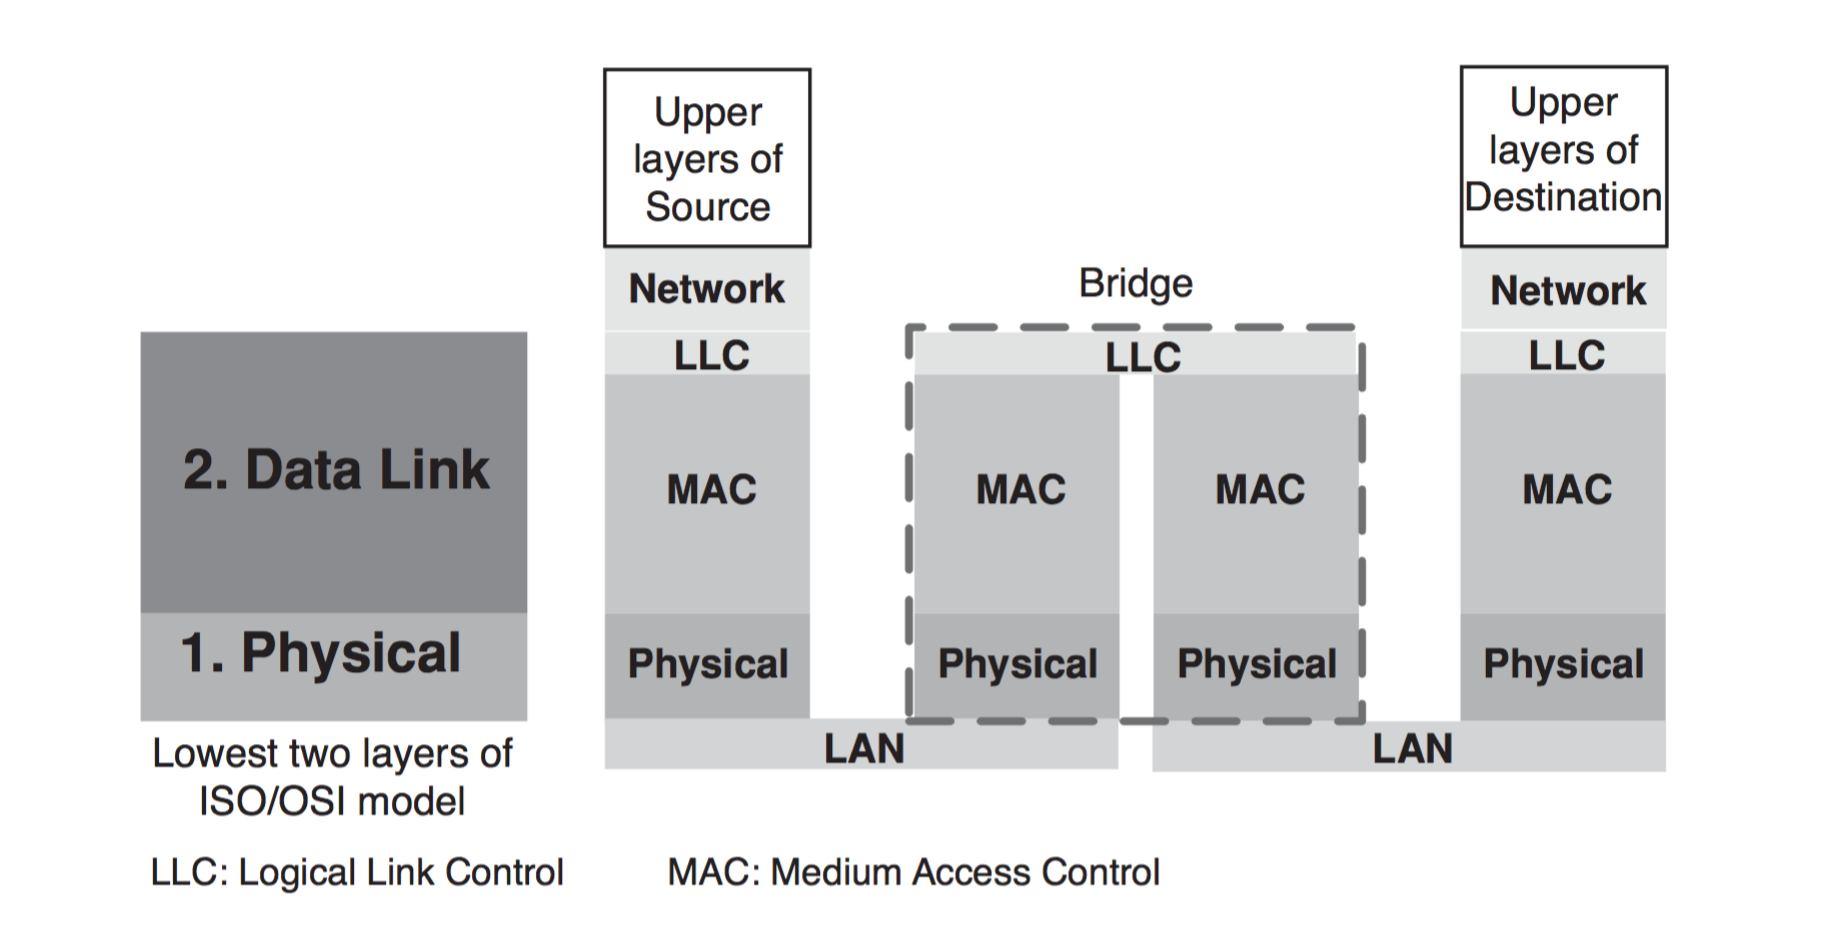
\includegraphics[scale=0.3,cfbox=blue_slides 1pt 0pt]{imgs/arch_ieee802.png}
		%\caption{Architettura IEEE 802}
	\end{figure}
\end{frame}

\begin{frame}{IEEE 802[.3]}
	\textbf{Ethernet}
	\begin{itemize}
		\item Una tra le tecnologie di rete più utilizzate per le LAN cablate
		\item Frame-based
		\item Utilizza un mezzo condiviso (collisioni gestite da \textit{CSMA/CD})
	\end{itemize}
	\begin{figure}[h] 
		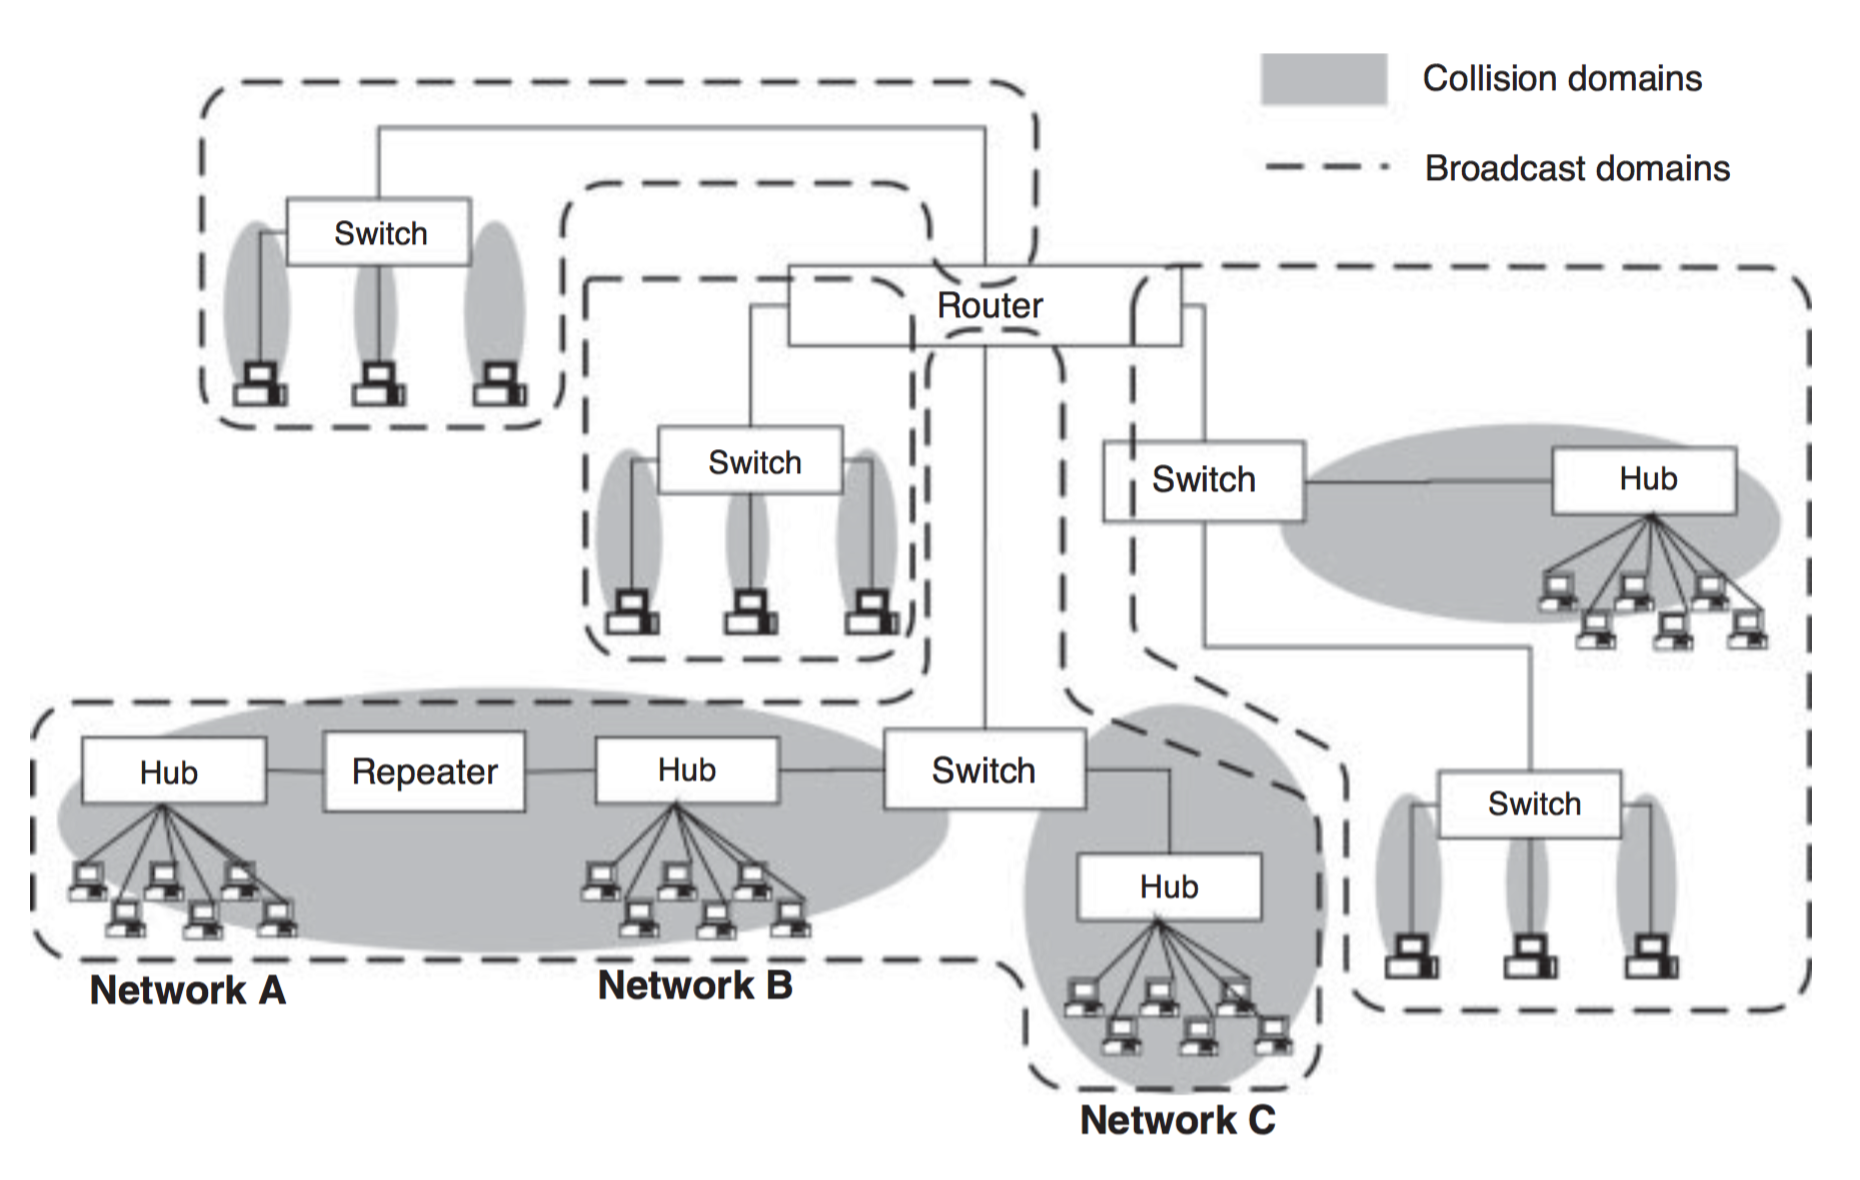
\includegraphics[scale=0.23,cfbox=blue_slides 1pt 0pt]{imgs/lan.png}
		%\caption{LAN Ethernet}
	\end{figure}
\end{frame}

\begin{frame}{IEEE 802[.11]}
	\textbf{Wireless}
	\begin{itemize}[<+- | alert@+>]
		\item Definisce un insieme di standard per le Wireless LAN
		\item Utilizza un mezzo condiviso (collisioni gestite da \textit{CSMA/CA})
		\item Componenti:
			\begin{itemize}
				\item Station
				\item Access Point (\textbf{BSS})
				\item Distribution System (\textbf{ESS})
			\end{itemize}
	\end{itemize}
\end{frame}
\begin{frame}{IEEE 802[.11]}
	\textbf{Wireless}
	\newline
	Basic Service Set (BSS)
		\begin{figure}[h] 
			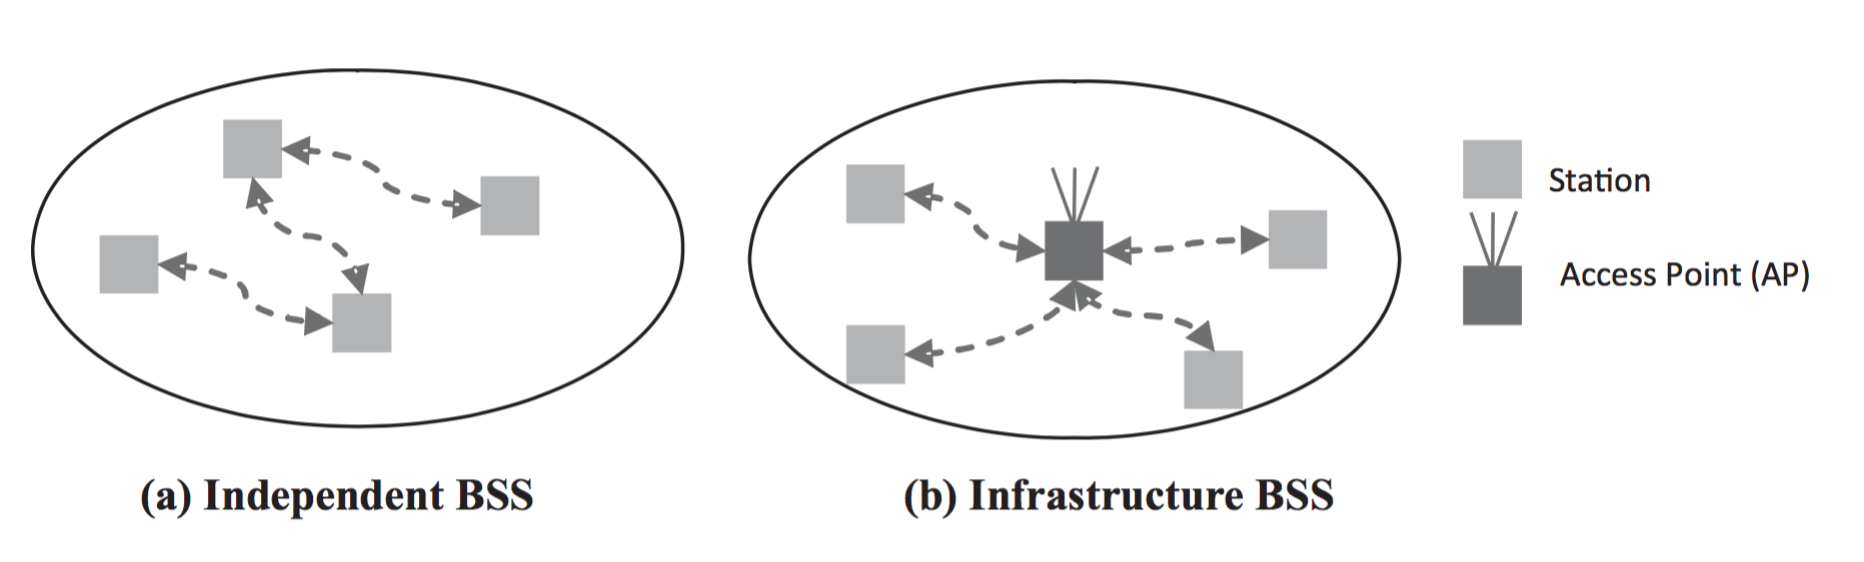
\includegraphics[scale=0.3,cfbox=blue_slides 1pt 0pt]{imgs/bss.png}
			%\caption{Architettura BSS}
		\end{figure}
	\end{frame}
	\begin{frame}{IEEE 802[.11]}
	\textbf{Wireless}
	\newline
	Distribution System
		\begin{figure}[h] 
			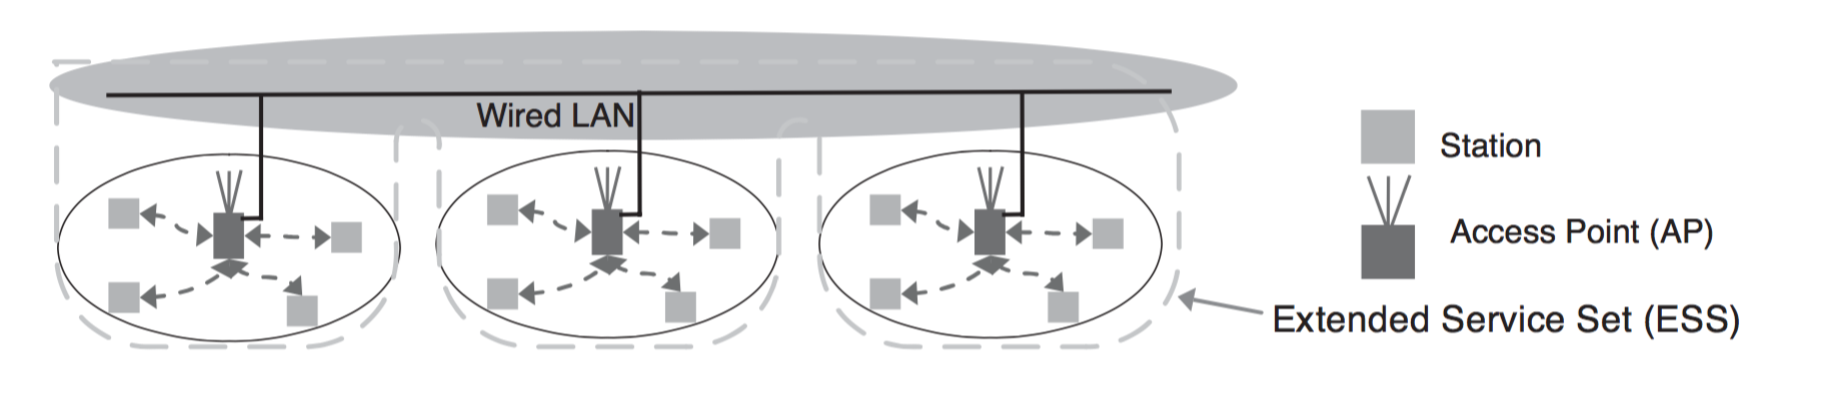
\includegraphics[scale=0.3,cfbox=blue_slides 1pt 0pt]{imgs/ds.png} %border color
			%\caption{Distribution System}
		\end{figure}
\end{frame}
	
\begin{frame}{IEEE 802[.15.1]}
	\textbf{Bluetooth}
	\begin{itemize}[<+- | alert@+>]
		\item Tecnologia wireless progettata per collegare dispositivi mobili o fissi
			\begin{itemize}[<+- | alert@+>]
				\item Bassi consumi
				\item Corto raggio d'azione
				\item Basso costo di produzione per dispositivi compatibili
			\end{itemize}
			\item Presenta due architetture di Rete
			\begin{itemize}[<+- | alert@+>]
				\item Piconet
				\begin{itemize}
					\item Un dispositivo \textit{Master}
					\item Fino a sette dispositivi \textit{Slave}
				\end{itemize}
				\item Scatternet
				\begin{itemize}[<+- | alert@+>]
					\item Un insieme di \textbf{Piconet}
				\end{itemize}
			\end{itemize}
	\end{itemize}		
\end{frame}

\begin{frame}{IEEE 802[.15.1]}
\textbf{Bluetooth}
	\begin{figure}[h] 
		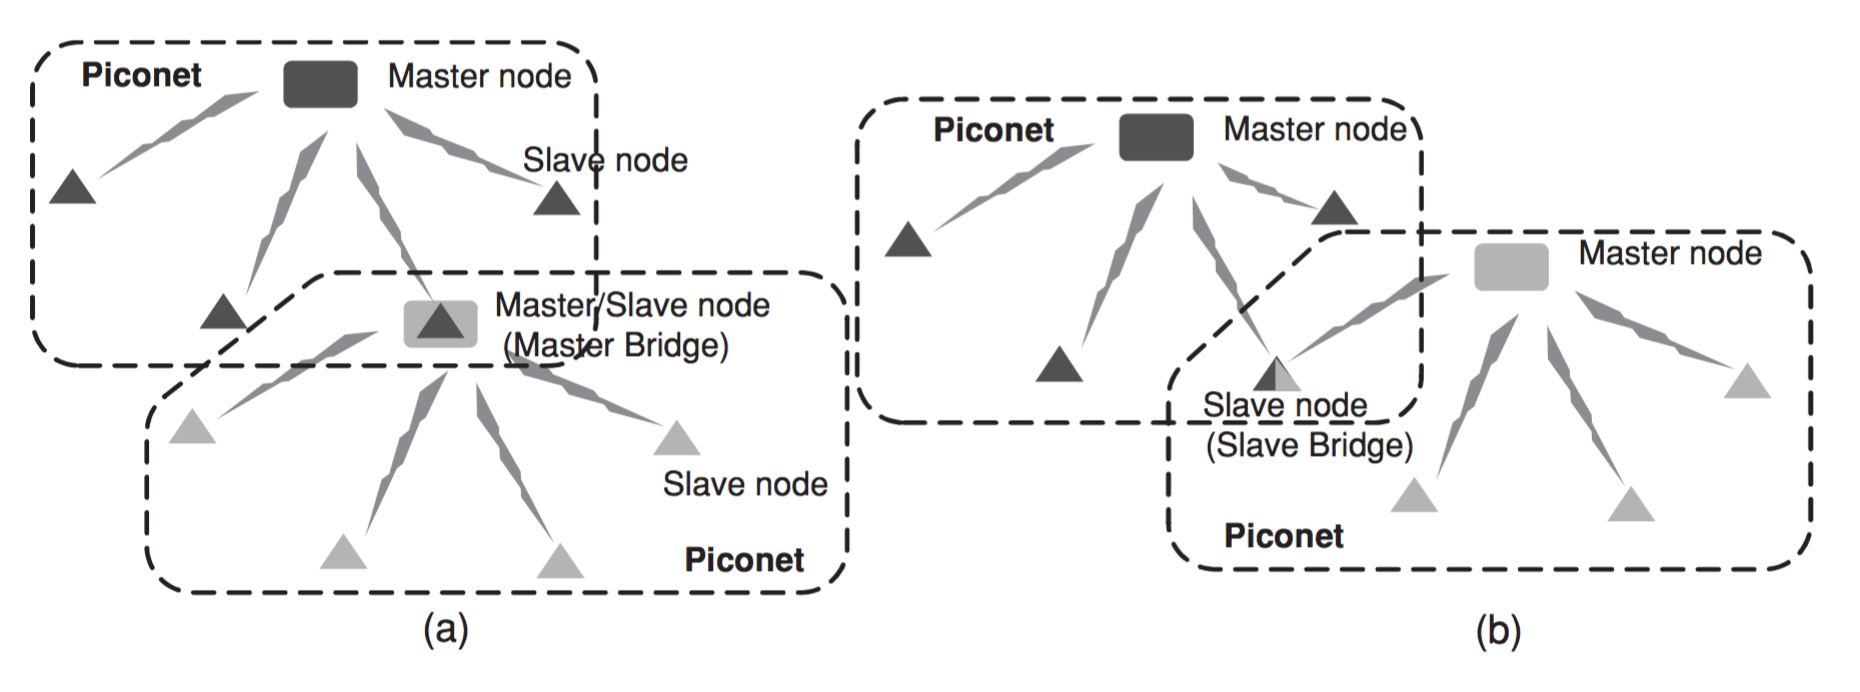
\includegraphics[scale=0.3,cfbox=blue_slides 1pt 0pt]{imgs/bt.png}
		%\caption{Piconet e Scatternet}
	\end{figure}
\end{frame}

%\begin{frame}{IEEE 802[.15.1]}
%\textbf{Bluetooth}
%\begin{itemize}[<+- | alert@+>]
%	\item Un dispositivo si può trovare in due stati
%	\begin{itemize}[<+- | alert@+>]
%		\item Connessione
%		\begin{itemize}[<+- | alert@+>]
%			\item Active mode
%			\item Hold mode
%			\item Sniff mode
%			\item Park mode
%		\end{itemize}
%		\item Standby
%		\begin{itemize}[<+- | alert@+>]
%			\item Ascolta il canale ogni 1,28 secondi per eventuali messaggi dal \textit{Master}
%		\end{itemize}
%	\end{itemize}
%\end{itemize}
%\end{frame}

\begin{frame}{IEEE 802[.15.4]}
\textbf{ZigBee \& 6LoWPAN}
	\newline
	Sono due tecnologie per Wireless Private Area Network (WPAN)
	\begin{itemize}[<+- | alert@+>]
		\item Basso consumo
		\item Alta flessibilità
		\item Bassi costi
	\end{itemize}
\end{frame}

\begin{frame}{IEEE 802[.15.4]}
\textbf{ZigBee}
%considerata come una buona opzione per il metering e per la gestione dell’energia ideale in implementazioni Smart Grid data la semplicità, mobilità, robustezza e i bassi costi di sviluppo.
%problematiche: basse capacità elaborative, piccola dimensione della memoria e interferenze.
\begin{itemize}
	\item \textit{Application Support} e \textit{Network Layer} sono definiti dalla ZigBee Alliance
	\item Un device può essere di due tipi
	\begin{itemize}
		\item Full Function Device (FFD)
			\begin{itemize}
				\item Coordinatore, Router, Device
				\item Può interagire sia con un FFD che con un RFD
			\end{itemize}
		\item Reduced Function Device (RFD)
			\begin{itemize}
				\item Device
				\item Può interagire solo con un FFD
			\end{itemize}
	\end{itemize}
\end{itemize}
	\begin{figure}[h] 
		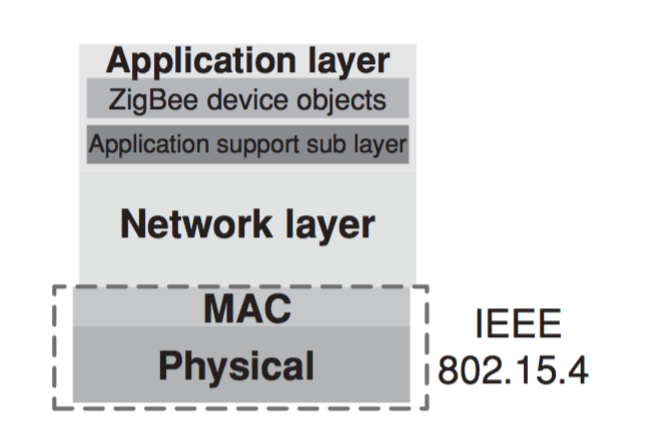
\includegraphics[scale=0.3,cfbox=blue_slides 1pt 0pt]{imgs/zbprot.png}
		%\caption{Architettura protocollare di ZigBee}
	\end{figure}
\end{frame}


%RFD vuole inviare un pacchetto al di fuori del dominio 6LoWPAN.
%RFD -> FFD(router) nella stessa WPAN -> gateway 6LoWPAN che inoltrerà al dispositivo destinatario tramite IP
\begin{frame}{IEEE 802[.15.4]}
	\textbf{6LoWPAN}
	\begin{itemize}
		\item Consente l'invio e la ricezione di pacchetti \textit{IPv6}
		\item E' stato inserito un Adaptation Layer per il collegamento tra lo strato \textit{MAC} e il \textit{Network Layer IPv6}
	\end{itemize}
	\begin{figure}[h]
		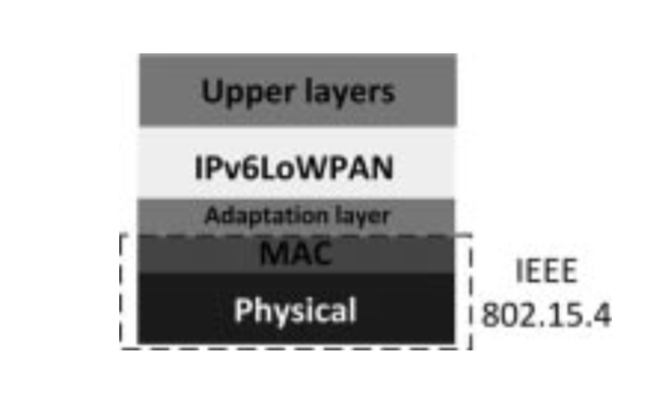
\includegraphics[scale=0.3,cfbox=blue_slides 1pt 0pt]{imgs/6pan.png}
		%\caption{Architettura di rete 6LoWPAN}
	\end{figure}
\end{frame}

\begin{frame}{IEEE 802[.16]}
	\textbf{WiMAX}
	\begin{itemize}[<+- | alert@+>]
		\item Tecnologia wireless adatta a trasmissione sia di tipo urbano che rurale
		\item Implementa diverse tecniche di crittografia, sicurezza ed autenticazione
		\item Tecnica di Orthogonal Frequency Division Multiple Access (OFDMA)
		\item Soddisfa varie specifiche imposte da una tipica Smart Grid
		%tra cui massima accessibilità ed interoperabilità, tempi di latenza inferiori ai 50 ms e larghezza di banda di 5 MHz.
		%\item La copertura si estende fino ai 50 km
		%\item Supporta i dispositivi mobili
	\end{itemize}
\end{frame}

\begin{frame}{IEEE 802[.16]}
	\textbf{WiMAX}
	\begin{figure}[h]
		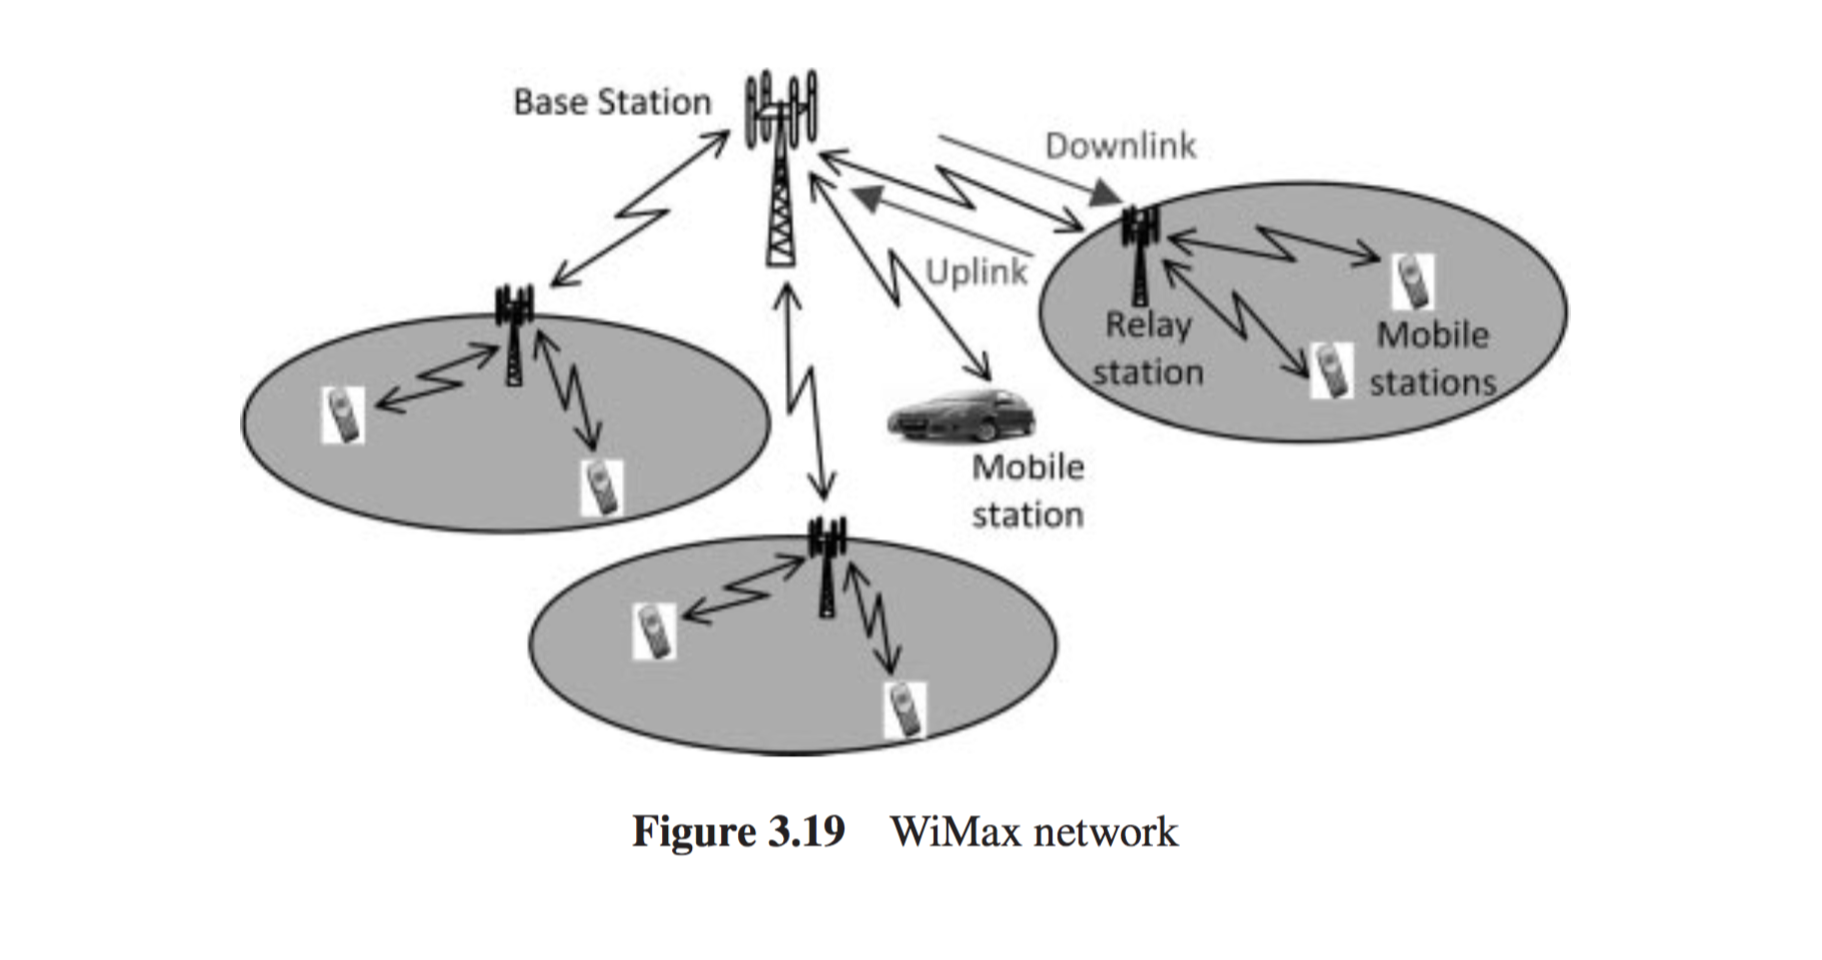
\includegraphics[scale=0.3,cfbox=blue_slides 1pt 0pt]{imgs/wim.png}
	\end{figure}
\end{frame}

%IEEE P1901 e HomePlug
\begin{frame}{Power line}
	\textbf{Power Line Communication}
	\begin{itemize}[<+- | alert@+>]
		\item Tecnologia di rete proposta per la trasmissione in ambiente Smart Grid
		\item Trasporto informazioni su conduttori e linee elettriche %risparmio dal punto di vista di creazione dell'infrastruttura
		\item Servizi di comunicazione per AMI e HAN
	\end{itemize}
	\pause
	\begin{block}{}
		\textit{In una tipica rete \textbf{\color{blue_slides}PLC}, gli smart meter sono collegati al data concentrator attraverso power line e i dati vengono trasferiti al data center tramite tecnologie di rete cellulare}
	\end{block}
	\pause
	\begin{block}{Problema}
		Presenza di disturbi che possono corrompere le informazioni, non garantendo più la continuità del servizio
	\end{block}
\end{frame}

\plain{Standard per lo scambio di informazioni}

\begin{frame}{Standard per lo scambio di informazioni}
	\textbf{Modbus}
	\begin{itemize}[<+- | alert@+>]
		\item Protocollo di messaggistica (\textit{Application Layer})
		\item Dispositivi collegati su diversi bus e reti
		\item Ethernet su fibra ottica con trasmissione seriale asincrona
		\item Automazione delle substation
		\item Comunicazione
			\begin{itemize}[<+- | alert@+>]
			\item Master $\xrightarrow{query}$ Slave/broadcast
			\item Slave (monitoring delle \textit{query})
			\item Slave $\xrightarrow{trigger}$ azione
			\end{itemize}
	\end{itemize}
\end{frame}

%\begin{frame}{Standard per lo scambio di informazioni}
%\textbf{DNP3}
%	\begin{itemize}[<+- | alert@+>]
%		\item Insieme di protocolli di comunicazione utilizzato tra i componenti nei sistemi di automazione
%		\item Fondamentale nei sistemi SCADA, utilizzato dalle Master Station per comunicare con le RTU e gli IED
%		%Lo User Layer DNP prende input analogici/binari e da in output segnali analogici e binari. Un master dnp3 invia richieste e le stazioni Slave rispondono, ma uno Slave può anche trasmettere messaggi senza aver ricevuto richiesta. Physical Layer utilizza noti protocolli di comunicazione seriali come EIA 232 o EIA 485.
%	\end{itemize}
%\end{frame}

\begin{frame}{Standard per lo scambio di informazioni}
	\textbf{ISO/IEC 61850}
	\begin{itemize}[<+- | alert@+>]
		\item Progettazione dei sistemi di automazione per le substation
		\item Sovrastruttura che coordina e gestisce protocolli e tecnologie esistenti
		\item Garantisce interoperabilità
	\end{itemize}
\end{frame}

\begin{frame}{Standard per lo scambio di informazioni}
	\textbf{ISO/IEC 61850}
	\begin{block}{Vantaggi}
	\begin{itemize}[<+- | alert@+>]
		\item Coordina la complessità di unità indipendenti
		\item Si integra con sistemi preinstallati in rete
		\item Scalabile e facilita integrazione
		\item Si basa su standard esistenti
		\item Supporta i \textit{self descriptive device}
		\item Si basa su \textit{data object}
		\item Estensibile e flessibile
		\item Si adatta rapidamente alla configurazione del sistema
	\end{itemize}
	\end{block}
\end{frame}


%Un device model considera inizialmente un physical device. Tale modello consente ad un singolo dispositivo fisico di agire da gateway di informazioni per più dispositivi. Successivamente vengono specificati i logical device all’interno di tale dispositivo. Ogni logical device contiene uno o più logical node, logicamente correlati ad una funzione della stazione. I logical node sono definiti da gruppi di data object e relativi servizi, ognuno modellato secondo gli schemi definiti dalle Common Data Classes (CDC).
\begin{frame}{Standard per lo scambio di informazioni}
\textbf{ISO/IEC 61850}
	\newline\textbf{Device Model}
%	\begin{itemize}
%		\item Physical Device
%		\item Logical Device
%		\item Logical Node
%			\begin{itemize}
%				\item Identificati con nomi definiti dallo standard in cui la prima lettera indica l'attinenza %A controllo automatico, M misura,etc.
%			\end{itemize}
%		\item Data Object e Servizi (\textit{Common Data Classes})
%	\end{itemize}
	\begin{figure}[h] 
		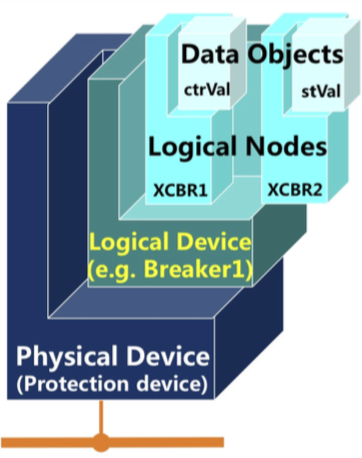
\includegraphics[scale=0.35,cfbox=blue_slides 1pt 0pt]{imgs/iec61850ln.png}
	\end{figure}
\end{frame}

\begin{frame}{Standard per lo scambio di informazioni}
\textbf{ISO/IEC 61850}
	\begin{itemize}[<+- | alert@+>]
		\item Oggetti e servizi astratti di comunicazione %permettono di scrivere un'applicazione indipendentemente dai protocolli tradizionali.
		\item Abstract Communication Service Interface (ACSI)
			\begin{itemize}[<+- | alert@+>]
				\item Oggetti e servizi implementati attraverso il protocollo Manufacturing Message Specification (MMS) %che definisce i messaggi di comunicazione tra i centri di controllo %o tra stazioni e centri
			\end{itemize}
		\item Linguaggio comune di configurazione per astrazione e standardizzazione
		\begin{itemize}[<+- | alert@+>]
			\item Substation Configuration Language (SCL)%basato su \textit{XML}
			\begin{itemize}[<+- | alert@+>]
			\item[+] Interoperabilità tra IED
			\item[+] Configurazione automatica
			\item[+] Riduzione della presenza di errori
			\end{itemize}
			\item Ogni IED presenta un file SCL che ne definisce la configurazione
		\end{itemize}
	\end{itemize}		
\end{frame}


%Spiegazione a voce
\begin{frame}{Standard per lo scambio di informazioni}
\textbf{ISO/IEC 61850}
\newline
Lo standard si serve dei seguenti strumenti per la gestione delle informazioni
\begin{itemize}[<+- | alert@+>]
	\item Generic Substation Event (GSE)
	\begin{itemize}[<+- | alert@+>]
		\item Generic Object Oriented Substation Event (GOOSE)
		\item Generic Substation State Event (GSSE)
	\end{itemize}
	\item Sampled Measured Values (SMV)
	\item Time Synchronization
	\item Report e Logging
\end{itemize}
\end{frame}

\plain{Standard per la sicurezza}

%\begin{frame}{Standard per la sicurezza}
%	\begin{itemize}[<+- | alert@+>]
%		\item Sono di recente invenzione e fondamentali data la grande mole di informazioni sensibili memorizzate sui computer collegati in rete
%		\item Molte attività si sono automatizzate introducendo maggiore bisogno di \textbf{\color{blue_slides}affidabilità} e \textbf{\color{blue_slides}sicurezza}
%	\end{itemize}
%\end{frame}

\begin{frame}{Standard per la sicurezza}
	\begin{block}{I problemi relativi alla sicurezza}
	\begin{itemize}
		\item[-] Accessi non autorizzati a informazioni recuperate dagli smart meter
		\item[-] Spegnimento di dispositivi
		\item[-] Attacco alla Smart Grid per causare un'interruzione al regolare passaggio di corrente
	\end{itemize}
	\end{block}		
	\pause
	\begin{block}{I problemi relativi alla privacy}
	\begin{itemize}
		\item[-] Alta frequenza di letture per misurare il consumo energetico
		\item[+] Si cerca di aggregare le informazioni per mascherare i singoli consumi dei meter
	\end{itemize}
	\end{block}		
\end{frame}

\begin{frame}{Standard per la sicurezza}
\textbf{ISO/IEC 62351}
\begin{block}{Obiettivi di sicurezza}
\begin{itemize}[<+- | alert@+>]
	\item Autenticazione nel processo di trasferimento di dati tramite firma digitale
	\item Garanzia di accessi esclusivamente dopo autenticazione
	\item Prevenzione dell'\textbf{\color{blue_slides}eavesdropping}
	\item Prevenzione da attacchi di \textbf{\color{blue_slides}playback} e attacchi di \textbf{\color{blue_slides}spoofing}
	\item Rilevamento delle intrusioni
\end{itemize}
\end{block}
\end{frame}

\begin{frame}{Standard per la sicurezza}
	\textbf{ISO/IEC 62351}
	\newline
	E'suddiviso in 8 parti:
	\begin{enumerate}[<+- | alert@+>]
		\item Spiegazioni di alcuni scenari
		\item Definizioni di termini
		\item Definizioni di servizi di sicurezza in comunicazione TCP/IP based
		\item Aumento dei messaggi di sicurezza trasmessi su MMS
		\item Procedure relative a Transport e Application Layer (TLS)%in modo da proteggere le informazioni trasmesse, riguarda invece la comunicazione seriale in cui si vanno a definire ulteriori misure di sicurezza per proteggere l’integrità delle connessioni seriali applicando chiavi hash
		\item ISO/IEC 61850 %profili per la comunicazione non basati su TCP/IP
		\item Network Management
		\item Role-Based access control
	\end{enumerate}
\end{frame}